\chapter{Introduction}

\section{Learning Technology}

% WHAT SHOULD GO HERE?
% Introduction to spaced repetition
% Survey of learning technologies used
% Gamification explained, stigma, some stuff about Skinner maybe?

\par Learning technology is becoming nearly universally used in classrooms, to the point where some teachers refer to it as "mandatory." \cite{BJET:BJET12051} Yet there is still a "great variation in university lecturers' use of technology," with some teachers not even ready to replace their overhead slides with Powerpoint.

\par We will address the different methodologies teachers use to integrate technology with the classroom, paying special attention to gamification techniques and spaced repetition.

\section{Definitions}

\subsection{Spaced Repetition}

\par In this paper, we introduce \textit{Commit}, a novel web-based application that uses spaced repitition and gamification elements to educational courses. For this thesis, \textit{Commit} was deployed to a variety of classes at California Polytechnic State University to measure its effect on student engagement and learning.

\subsection{Why College Classes?}
\par \textit{Commit} was tested with classes at California Polytechnic State University to facilitate the creation of questions and evaluation of the application. While the app would work with any level of education from K-12 to higher education, using Cal Poly classes allowed us to easily create questions for classes that we had just taken

%\par Gamifying in education has several hurdles. Gamification tends to come with a negative stigma; teachers often feel that gamified services aren't as "serious" as other learning technologies. In addition, existing education gamification solutions have usability issues and are not accessible to students that don't have a background in videogames.

\section{Spaced Repetition}
\par One of the key aspects of Commit is its use of spaced repetition. Spaced repetition is an idea first brought into the mainstream by Pimsleur in the 1960s. Spaced repetition is a learning technique where students reinforce learned knowledge at specific intervals, improving long-term retention and recall ability.

\begin{figure}[h]
	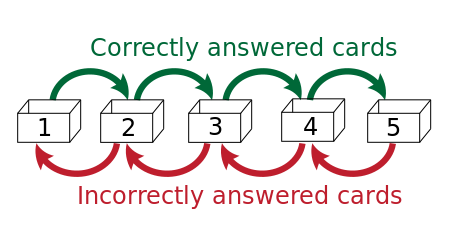
\includegraphics{figures/leitner}
	\caption{The Leitner system. If a student answers a flashcard correctly, it is moved to a higher-numbered box that is reviewed less frequently.}
	\label{fig:leitner}
\end{figure}

\par A simple example of spaced repitition is known as the Leitner system. Flashcards are organized into numbered boxes. (See \textbf{\hyperref[fig:leitner]{Figure \ref*{fig:leitner}}}). Each successive box is reviewed less frequently. That is, a student would review Box 1 twice per day, Box 2 once per day, Box 3 every 2 days, and so on. If a card is answered correctly, it is moved to a box that is reviewed less frequently. However, if the student answers incorreclty, the card is moved to a box that is reviewed more frequently.

\par Thus, tougher cards are reviewed more often, and cards the student knows will be reviewed less often. However, all cards are \textit{eventually} reviewed, and even cards that the student always answers correctly are reviewed in the long term.

\par There is strong evidence that this idea of "spaced repitition" enhances long-term memory and deepens understanding of subject material. \cite{edge2012memreflex}

%[http://www.memorylifter.com/fileadmin/publications/Spacing_Effect_and_Mnemonic_Strategies.pdf]

\section{Spaced Repitition Apps}
\subsection{Duolingo}

\begin{figure}
	%\centering
	\centerline{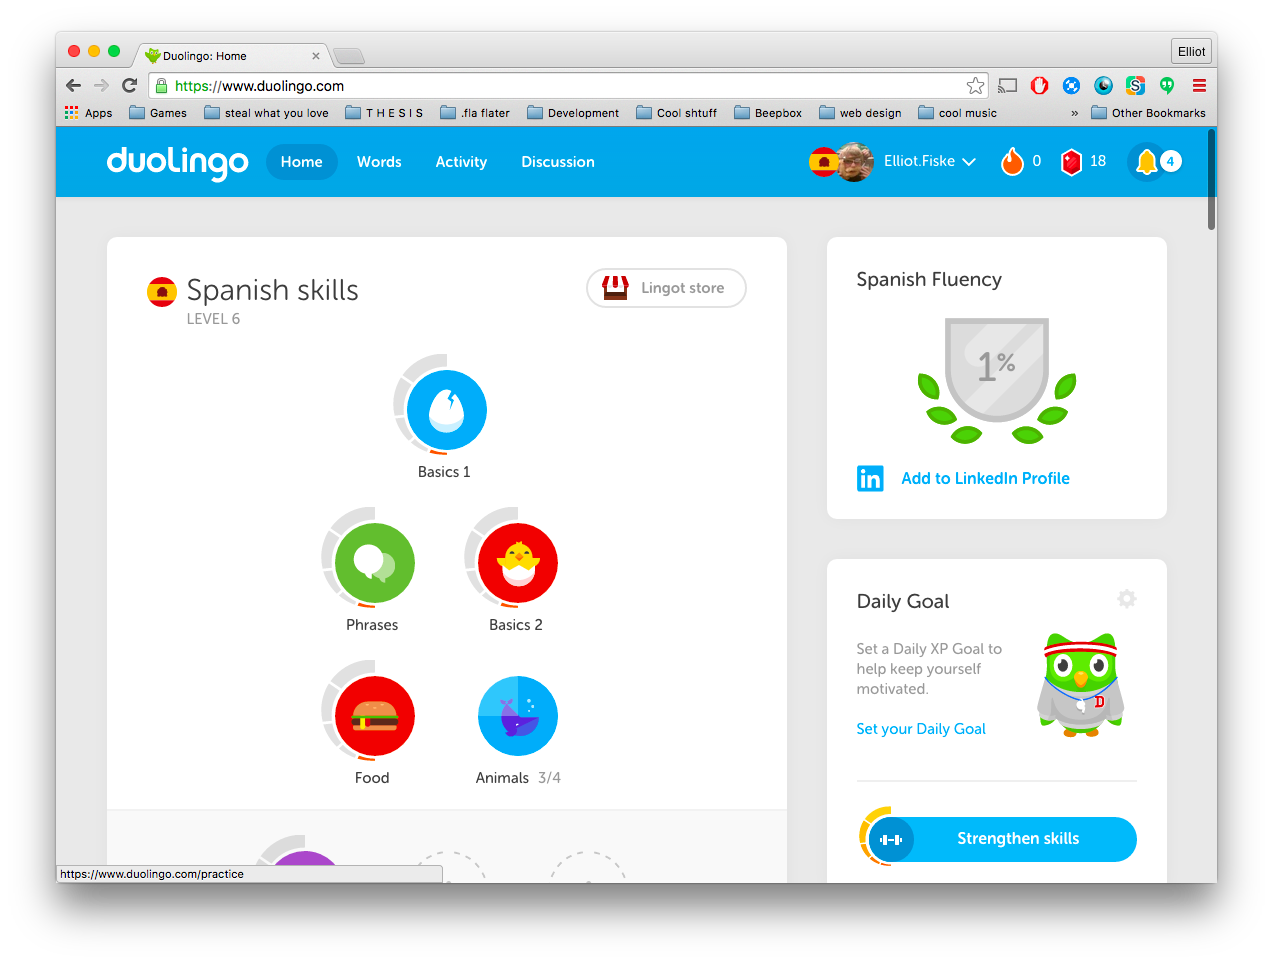
\includegraphics[width=1.2\linewidth]{duolingo}}
	\caption[Duolingo]{The Duolingo interface. Notice the gamification elements and the encouragement to reach a "daily goal."}
	\label{fig:duolingo}
\end{figure}

\par Several recent apps and products make use of spaced repitition to allow user to easily gain long-term recall of languages, class content, or any other information that needs to be learned. One such app is Duolingo (See \textbf{\hyperref[fig:duolingo]{Figure \ref*{fig:duolingo}}}); in Duolingo, users learn a language by repeating small tasks every day. 

\par The app encourages users to spend a small amount of time each day studying useful words and phrases, rather than cramming in a lot of knowledge at once. It encourages this behavior through the use of gamification. Each user earns "experience" in a language, eventually leveling up. Users connect their Facebook accounts and can see their friends' levels and accomplishments, adding a social element to the app.

\subsection{Memrise}

\begin{figure}
	\centering
	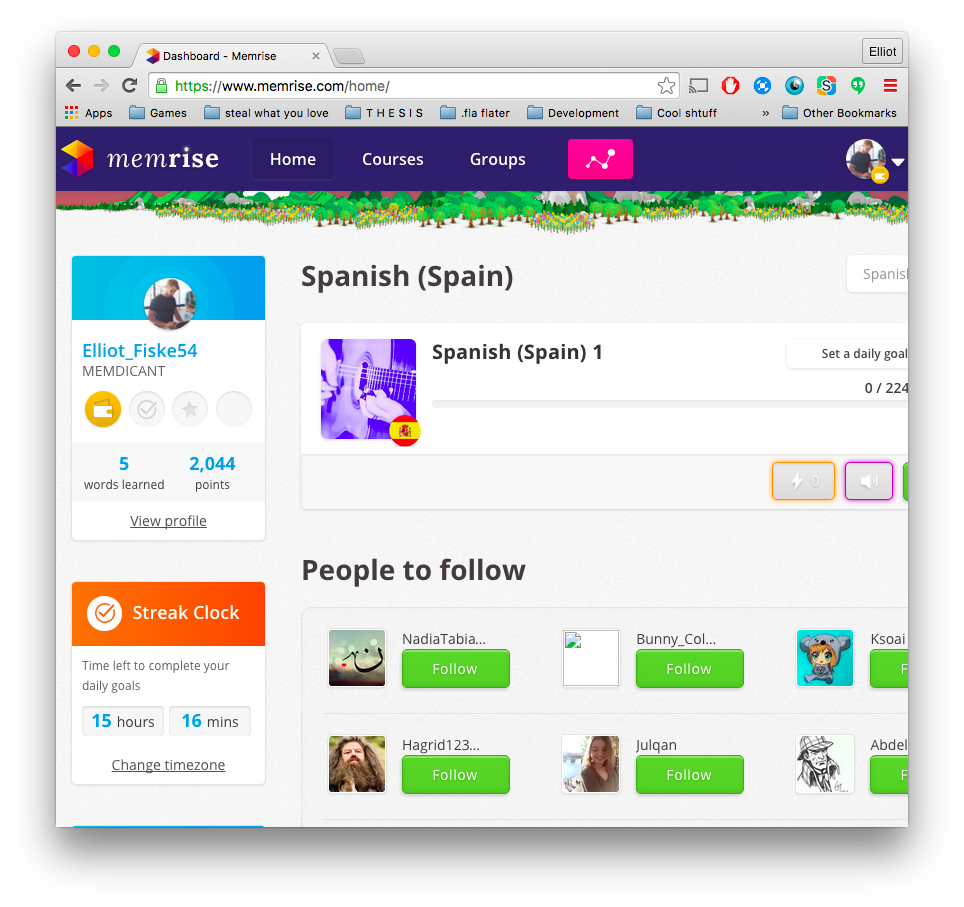
\includegraphics[width=0.7\linewidth]{memrise}
	\caption[Memrise]{Screenshot of the Memrise interface. Note the gamification elements, the social aspect, and the "Streak" clock encouraging consistent use of the app.}
	\label{fig:memrise}
\end{figure}

\par Memrise (See \textbf{\hyperref[fig:memrise]{Figure \ref*{fig:memrise}}})is a web app that has very similar function to \textit{Commit.} Memrise takes a series of flashcard-based questions and answers and automatically creates a "study plan" where the application breaks up flash cards and uses spaced repitition to encode the information in the user's long-term memory. Memrise also uses gamification and social elements, as users earn points for every correct answer and can see their friends' scores.

\par Interesting to note is that users can input any data they choose into Memrise to receive a custom study-guide. This would allow students to easily learn flashcards if they took the time to input them into the app.

\par Both of these applications heavily emphasize language learning, since the process of learning a language can easily be broken down into a series of small words and phrases, and re-emphasized using the process of spaced repitition. However, Commit is scoped specifically to one class, allowing students to easily learn and retain class content without the commitment of adding their own flashcards.

\section{Gamification}
\par The \textit{Commit} app is structured to incentivize students to enjoy using it. The primary incentive for experimental participants was the chance at winning a \$20 Amazon gift card. However, in order to actually obtain this reward the participants would have to engage with the app's systems.

\par One powerful technique used by Commit is the idea of variable rewards scheduling. Variable rewards scheduling is based off of the idea that it's boring to always receive the same reward for performing the same action. It's far more exciting and engaging to not know what reward you'll receive; several studies affirm that variable reward scheduling leads to more willingness to perform a desired target action \cite{dodin2001integrated}.

\par In order to earn entries into the \$20 gift card raffle, participants are required to earn a certain number of \textbf{points.} These points are earned through answering questions. However, far more points are earned if the user returns to the app every day. In addition, "bonus rewards" will be awarded at random intervals to engage users more. The expectation that today may be the "bonus reward" day leads to greater user engagement with the system.

\par In general, users reported that they enjoyed the gamification sections and the potential to earn rewards. Through the study in general, we note that users showed higher rates of engagement and improvements in test scores over the control group that did not use the app.